\Chapter{Mintafeladat bemutatása}
Az alábbiakban egy mintafeladat bemutatására kerül sor. A mintafeladat egy nagyon egyszerű BPEL példa. Egyszerűségét az indokolja, hogy a forrás file-nak és az elkészült hálónak is bele kell férni (olvashatóan) egy A4-es lap kereteibe. Továbbá, az egyszerűség segíti a megértést is.

\Section{A forrás file}

Vegyük az alábbi forrást:

\begin{cpp}
<?xml version="1.0" encoding="utf-8" ?>
<bpel:process name="hworld"
 targetNamespace="http://eclipse.org/bpel/sample"
 suppressJoinFailure="yes"
 xmlns:tns="http://eclipse.org/bpel/sample"
 xmlns:bpel="http://docs.oasis-open.org/wsbpel/2.0/process/executable"
 >
  <bpel:import location="hworldArtifacts.wsdl" 
	namespace="http://eclipse.org/bpel/sample"
	importType="http://schemas.xmlsoap.org/wsdl/" />

  <bpel:partnerLinks>
   
    <bpel:partnerLink name="client"
                 partnerLinkType="tns:hworld"
                 myRole="hworldProvider"
                 partnerRole="hworldRequester"
										 />
  </bpel:partnerLinks>
  <bpel:variables> 
    <bpel:variable name="input"
              messageType="tns:hworldRequestMessage"/>
    <bpel:variable name="output"
              messageType="tns:hworldResponseMessage"/>
  </bpel:variables>
  
  <bpel:sequence name="main">
    <bpel:flow name="mainFlow">
      <bpel:invoke name="flow1" operation="main1"/>
      <bpel:invoke name="flow2" operation="main2"/>
    </bpel:flow>
   
  </bpel:sequence>
  <bpel:sequence name="main1">
    <bpel:receive name="receiveInput" partnerLink="client"
           operation="initiate" variable="message"
           createInstance="yes"/>
  </bpel:sequence>

  <bpel:sequence name="main2">
    <bpel:send name="sendOutput" partnerLink="client"
               operation="initiate" variable="message"/>
  </bpel:sequence>
</bpel:process>
\end{cpp}

Ha megvizsgáljuk az inputot látjuk, hogy három szegmensből áll:
\begin{itemize}
\item \emph{Meta:} Ide kerülnek a file definíciós metaadatok, ezek a BPEL engine-nek szólnak, a konverzióhoz (talán a  név kivételével) szükségtelenek.
\item \emph{PartnerLinks} Partner linkek a BPEL folyamatok közötti összekötő eleme. Ha a konverzióhoz nem adunk meg adatokat a kapacitásokra, az elkészült hálóhoz, a partner link segítségével lehetne megtudni, milyen kapacitásokat kell az egyes node-okhoz rendelni. 
\item \emph{Sequence: Main} Mint a C típusú nyelvekben itt is a \emph{Main} a fő programszál. Alább felsorolható a többi segéd szál, illetve fölötte a változók, amiket a függvényeink, és különböző folyamatok használnak. 
\end{itemize}

A bemenetünket megvizsgálva látjuk, hogy ez maximum három szint mély XML file (a Main-re nézve). Erre azért van szükség, mert a BPEL támogatja a kvázi végtelen mélységű file generálását, viszont a legtöbb XML feldolgozó rutin nem tud kezelni nagyon mély dokumentumokat. Ez azzal magyarázható, hogy az XML-re ilyenkor inkább, mint egy adatleíró, adattároló dokumentumra tekintenek, mintsem egy kvázi programkódra. A programomban ezért kellett egy megkötést alkalmazni. A három szintű mélység fixálása jelentősen megkönnyíti az input feldolgozását. Szerencsére a fixálás könnyen kivitelezhető, ugyanis a BPEL-ben is támogatott a saját metódus írása. Itt ún. szekvenciákkal (\emph{sequence}) lehet ezeket leírni. A szekvenciákat pedig meg lehet hívni \emph{invoke}-kal.\\
A folyamat maga lebontva:
\begin{itemize}
\item A main folyamat indul el először. A folyamat elindít egy két ágú párhuzamosítást a \emph{flow}-al
\item A \emph{flow} két ágában egy-egy \emph{invoke} meghívja a megfelelő szubrutint.
\item A \emph{main1} szubrutin majd rögtön elkezd várakozni egy üzenetre.
\item A \emph{main2} az előbb említett szubrutin számára küldi az üzenet tokent. 
\end{itemize}

\Section{Az elkészült színes háló}
Most, hogy láttuk a bemenetet, a programot "színes" módra kapcsolva nézzük meg az általa generált hálót.
A program a következő hálót generálja: \ref{fig:demo} 

\begin{figure}[h!]
\centering
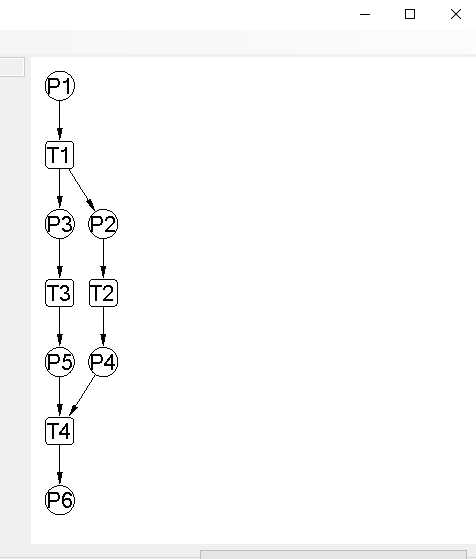
\includegraphics[scale=0.6]{images/demo2.png}
\caption{A generált mintaháló}
\label{fig:demo}
\end{figure}

A hálókba a tranziciók lekerekített sarkú téglalappal, lettek jelölve, a szokásos fekete téglalap helyett. Erre azért van szükség mert a tranzició így a gráfon belül elnevezhető. Előre láthatólag a hálóban kettő token lesz. Az egyik a vezérjel, a másik pedig az üzenet. A vezérjel token mindenhol előfordul és kapacitása mindenhol $1$. Ha ettől kevesebbszer fordul elő, az azt jelenti, hogy ott még nem tart a végrehajtás. Többször nem fordulhat elő, ugyanis azt egy adott tranzició majd elnyeli végrehajtáskor.
Vegyük észre, hogy a "P6" helyre csak "T4" en keresztül kerülhet vezérjel. A T4 pedig üzenetet vár "P4" től, ezért "AND" módban működik.   

A láthatjuk a VS debug segítségével, hogy a hálót graph-builder az alábbi módon rakja össze a háttérben:
\begin{verbatim}
graph.AddEdge("P1", "T1");
graph.AddEdge("T1", "P2");
graph.AddEdge("T1", "P3");
graph.AddEdge("P2", "T2");
graph.AddEdge("P3", "T3");
graph.AddEdge("T2", "P4");
graph.AddEdge("T3", "P5");
graph.AddEdge("P4","T4");
graph.AddEdge("P5","T4");
graph.AddEdge("T4","P6");
graph.FindNode("P1").Attr.Shape = Shape.Circle;
graph.FindNode("P2").Attr.Shape = Shape.Circle;
graph.FindNode("P3").Attr.Shape = Shape.Circle;
graph.FindNode("P4").Attr.Shape = Shape.Circle;
graph.FindNode("P5").Attr.Shape = Shape.Circle;
graph.FindNode("P6").Attr.Shape = Shape.Circle;
graph.FindNode("T1").Attr.Shape = Shape.Box;
graph.FindNode("T2").Attr.Shape = Shape.Box;
graph.FindNode("T3").Attr.Shape = Shape.Box;
graph.FindNode("T4").Attr.Shape = Shape.Box;
\end{verbatim}

\Section{Kapacitás elemzés}
Sajnos az egy A4-es oldalon olvashatóan megjeleníthető hálók mérete korlátos. Ezért a példa során kompromisszumot kellett kötni, vagy egy olyan példát mutatok be, amin érdekes kapacitást számolni a sok különböző token miatt, de nem fér ki egy lapra csak részleteiben, vagy pedig egy egyszerűbb, hálót ami valószínűleg nem fog kapacitás korlátot generálni. 
A kapacitás számítás egy másik hálóra úgy történne, hogy az elkészült háló generálása után, meg kell adni a helyek és tranziciók paramétereit kézzel. A koverzió során ugyanis egy segéd fileból olvasható be a szükséges kapacitás, ami eredetileg szintén BPEL file lenne. A több file-os összeolvasás viszont jelentősen megnöveli a program komplexitását, és gyakorlatilag egy BPEL compiler lenne az elkészült program. Ezt egy szakdolgozati időkeretben lefejleszteni sajnos elég nehézkes, ezért maradtam a külső file-os kapacitásnál. 

